\section{Cofibrations}
For this section, we will follow chapter VII.1 in \cite{Bredon}.\\
\linebreak
One of the fundamental questions in topology is the
"extension problem". Namely, given a map
$g \colon A \to Y$ defined on a subspace $A$ of $X$, when
can we extend this map to all of $X$.

This cannot always be done - for example, as is the case
with $A = Y = S^{n}$ and $X = D^{n+1}$ choosing the
map to be any degree $-1$ map.\\
\linebreak
\begin{question}
    Is the extension problem a \textit{homotopy-theoretic} problem?
    That is, does the answer depend only on the homotopy
    class of $g$?
\end{question}
The answer is: generally not. 
For example, we can take $X = \left[ 0,1 \right] ,
A = \left\{ 0 \right\} \cup \left\{ \frac{1}{n} \mid 
n=1, 2, \ldots \right\} $ and $Y = CA$, the cone
on $A$. Choosing $g$ to be the inclusion of
$A$ into $Y$, this cannot be extended to $X$ as the
extension would be discontinuous at $\left\{ 0 \right\} $.
However, $g \simeq g'$ with $g'$ being the constant
map of $A$ to the vertex of the cone, and $g'$ easily
extends to $X$ by the constant map.\\
\linebreak
It turns out, however, that under some very mild conditions
on the spaces, the problem becomes homotopy theoretic. 
We will now discuss this.

\begin{definition}[Homotopy extension property]
    Let $\left( X,A \right) $ and $Y $ be given spaces.
    Then $\left( X, A \right) $ is said to have
    the \textit{homotopy extension property} with respect to
    $Y$ if the following diagram can always be completed
    to be commutative.
    \begin{equation*}
    \begin{tikzcd}
        A \times I \cup X \times \left\{ 0 \right\} 
        \ar[r] \ar[d, hookrightarrow] & Y\\
        X \times I \ar[ru, dashed]
    \end{tikzcd}
    \end{equation*}

    One can also depict this by the following diagram:
    \begin{equation*}
    \begin{tikzcd}
        A \times \left\{ 0 \right\} \ar[rr, hookrightarrow]
        \ar[dd, hookrightarrow] 
        & & A \times I \ar[dd, hookrightarrow] \ar[ld] \\
        & Y & \\
        X \times \left\{ 0 \right\} \ar[ru] \ar[rr] && X \times I
        \ar[lu, dashed]
    \end{tikzcd}
    \end{equation*}
\end{definition}

If $\left( X,A \right) $ has the homotopy extension property
with respect to $Y$, then the extensibility of maps
$g \colon A \to Y$ depends only on the homotopy class of
$g$. For suppose $H \colon g \simeq g'$ and $g'$ can be
extended to  $\tilde{g'} \colon X \to Y$, 
then define the map
$A \times I \cup  X \times \left\{ 0 \right\} $ by
$\tilde{g'} \times \left\{ 0 \right\} $ on
$X \times \left\{ 0 \right\} $ and
$H$ on $A \times I$. The homotopy extension property for the
pair $(X,A)$ then guarantees the existence of a map
$G \colon X \times I \to Y$ which equals
$g$ on $A \times \left\{ 1 \right\} $, so
$H \left( -,1 \right) \colon X \to Y$ extends $g$.

\begin{definition}[Cofibration]
    Let $f \colon A \to X$ be a map. Then $f$ is called
    a \textit{cofibration} if one can always fill in the following
    commutative diagram given the solid arrows:
    \begin{equation*}
    \begin{tikzcd}
        A \times \left\{ 0 \right\} \ar[dd, "f \times \id"] 
        \ar[rr, hookrightarrow]
        & & A\times I \ar[dd, "f \times \id"] \ar[dl] \\
            & Y &\\
        X \times \left\{ 0 \right\} \ar[ru]
        \ar[rr, hookrightarrow]& & X \times I 
        \ar[lu, dashed]
    \end{tikzcd}
    \end{equation*}
    for \textit{any} space $Y$.
\end{definition}

\begin{note}
    If $f$ is an inclusion, the this is the same
    as the homotopy extension property for all $Y$. That attribute
    is sometimes referred to as the 
    \textit{absolute homotopy extension property}.
\end{note}

\begin{lemma}[]\label{Lemma:Cofibration-Inclusion-2}
    If $f \colon A \to X$ is a cofibration, then
    the inclusion  $\iota \colon f(A) \hookrightarrow X$ 
    is a cofibration with $f\left( A \right) $ inheriting
    the subspace topology.
\end{lemma}

\begin{proof}
    If $f$ is a cofibration, then for any $Y$, there
    following diagram can be filled out given the solid arrows

    \begin{equation*}
    \begin{tikzcd}
        A \times \left\{ 0 \right\} \ar[dd, "f \times \id"] 
        \ar[rr, hookrightarrow]
        & & A\times I \ar[dd, "f \times \id"] \ar[dl] \\
            & Y &\\
        X \times \left\{ 0 \right\} \ar[ru]
        \ar[rr]& & X \times I 
        \ar[lu, dashed, "F"]
    \end{tikzcd}
    \end{equation*}
    And thus we can fill the following diagram as well

    \begin{equation*}
    \begin{tikzcd}
        f(A) \times \left\{ 0 \right\} \ar[dd, "\iota \times \id",
        hookrightarrow] 
        \ar[rr, hookrightarrow]
        & & f(A) \times I \ar[dd, "\iota \times \id", 
        hookrightarrow, bend left] \ar[dl, "F|_{f(A) \times I}"] \\
            & Y &\\
        X \times \left\{ 0 \right\} \ar[ru]
        \ar[rr, hookrightarrow]& & X \times I 
        \ar[lu, dashed, "F"]
    \end{tikzcd}
    \end{equation*}
    By definition then $\iota \colon
    f(A) \hookrightarrow X$ is a cofibration.
\end{proof}

\begin{note}
    Note that the converse is not true since
    we will see later in a problem that
    a cofibration is an embedding, so it is
    easy to construct a counter example, for example
    by choosing a well-pointed space (see definition later)
    and then choosing any space
    $A$ which is not a single point and the collapsing map
    $A \to X$ to the base point.
\end{note}

\begin{theorem}[]\label{Thm:Retract-cofibration}
    For an inclusion $A \subset X$, the following are equivalent:
    \begin{enumerate}
        \item The inclusion map $A \hookrightarrow X$ is a 
            cofibration.
        \item $A \times I \cup  X \times  \left\{ 0 \right\} $ 
            is a retract of $X \times I$.
    \end{enumerate}
\end{theorem}

\begin{proof}
    If the inclusion is a cofibration, then choosing
    $Y = A \times I \cup  X \times \left\{ 0 \right\} $ 
    with all arrows being inclusions in the
    diagram of a cofibration, we obtain a map
    $X \times I \to A \times I \cup  X \times \left\{ 0 \right\} $ 
    which is the identity on
    $A \times I \cup  X \times \left\{ 0 \right\} $.\\
    Conversely, if $A \times I \cup  X \times \left\{ 0 \right\} $ 
    is a retract of $X \times I$, then
    we can always complete the diagram by
    mapping $X \times I \to 
    A \times I \cup  X \times  \left\{ 0 \right\} 
    \to Y$ where the second map
    takes the maps $A \times I \to Y$ and
    $X \times \left\{ 0 \right\} \to Y$ from the diagram.
\end{proof}

\begin{corollary}\label{Cor:Subcomplex-Cofibration}
    If $A$ is a subcomplex of a CW-complex $X$, then
    the inclusion $A \hookrightarrow X$ is a cofibration.
\end{corollary}

\begin{proof}
    We want to construct a retraction
    $X \times I \to A \times I \cup  X \times \left\{ 0 \right\} $.
    We will do so by constructing a retraction
    $\left( \left( A \cup X^{(r)}  \right)\times I  \right) \cup 
    \left( X \times \left\{ 0 \right\}  \right) 
    \to \left( A \times I \right) \cup \left( X \times 
    \left\{ 0 \right\} \right) $ by induction on $r$.
    If it has been defined on the
    $(r-1)$-skeleton, then extending it over an
    $r$-cell is simply a matter of extending a map
    on $S^{r-1} \times I \cup D^{r} \times \left\{ 0 \right\} $ 
    over $D^{r} \times I$ which can be done
    since the pair
    $\left( D^{r} \times I, S^{r-1} \times I
    \cup D^{r} \times \left\{ 0 \right\} \right) $ is homeomorphic
    to $\left( D^{r} \times I, D^{r}\times \left\{ 0 \right\} 
    \right) $.
    See Figure \ref{fig:DUWUWUJK122-png}

    \begin{figure}[htpb]
        \centering
        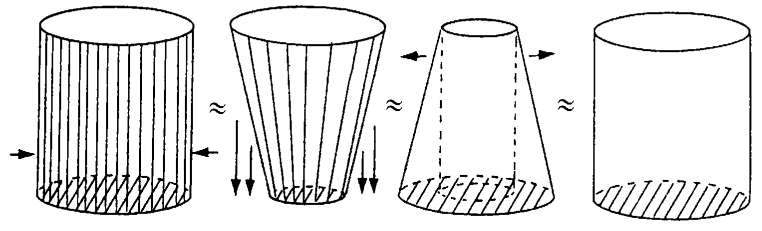
\includegraphics[width=0.8\textwidth]{Figures/DUWUWUJK122.png}
        \caption{A homeomorphism of pairs.}
        \label{fig:DUWUWUJK122-png}
    \end{figure}
    These maps for each cell fit together to
    give a map on the $r$-skeleton because of the
    weak topology on $X \times I$. The union of these
    maps for all $r$ gives a map on $X \times I$, again because
    of the weak topology on $X \times I$.
\end{proof}

\begin{theorem}[]\label{Thm:SJJDHW29WW}
    Assume that $A \subset X$ is closed and that there
    exists a neighborhood $U$ of $A$ and a map
    $\varphi  \colon X \to I$ such that
    \begin{enumerate}
        \item $A = \varphi ^{-1} (0)$.
        \item $\varphi \left( X-U \right) = \left\{ 1 \right\} $.
        \item $U$ deforms to $A$ through $X$ with $A$ fixed.
            That is, there is a map $H \colon U \times I \to X$ 
            such that $H(a,t) = a$ for all $a \in A, H
            (u,0) = 0$, and $H(u,1) \in A$ for all $u \in U$.
    \end{enumerate}
    Then the inclusion
    $A \hookrightarrow X$ is a cofibration. The converse also
    holds.
\end{theorem}

\begin{proof}
    We may assume that $\varphi  = 1$ on a neighborhood
    of $X - U$ by replacing $\varphi $ with
    $\min \left( 2 \varphi , 1 \right) $.
    It suffices to show that there exists a retract
    $\Phi \colon U \times I \to X \times \left\{ 0 \right\} 
    \cup A \times I$ since then the
    map
    \[
    r\left( x,t \right) 
    =
    \begin{cases}
        \Phi\left( x, t \left( 1-\varphi (x) \right)  \right),&
        x \in U\\
        (x,0),& x \not\in U
    \end{cases}
    \] 
    gives a retraction $X \times I \to A \times I \cup 
    X \times \left\{ 0 \right\} $.\\
    We define $\Phi$ by
    \[
    \Phi(u,t) = 
    \begin{cases}
        H\left( u, \frac{t}{\varphi (u)} \right) \times 
        \left\{ 0 \right\},& \varphi (u) > t\\
        H\left( u,1 \right) \times 
        \left\{ t- \varphi (u) \right\} ,& \varphi (u)\le t.
    \end{cases}
    \] 
    The only thing that needs checking here is
    that $\Phi$ is continuous at
    points $\left( u,0 \right) $ such that
    $\varphi (u) = 0$, i.e., points $(a,0)$ for 
    $a \in A$ - indeed here the expression for
    $\varphi (u) > t$ is not defined.

    Recall that a map $f \colon X \to Y$ is continuous
    if for every point $x \in X$ and any neighborhood
    $U$ of $f(x)$, there exists a neighborhood
    $V$ of $x$ such that $f(V) \subset U$.\\
    So let $W$ be a neighborhood of $a = 
    H(a,t)$. Then there exists a neighborhood
    $V \subset W$ containing $a$ such that
    $H\left( V \times I \right) \subset W$, by
    assumption of $H$ being continuous.
    So for $t < \varepsilon$ for some $\varepsilon$ and
    $u \in V$, we have
    $\Phi \left( u,t \right) 
    \in W \times \left[ 0,\varepsilon \right] $.
    Hence $\Phi$ is continuous.\\
    \linebreak
    To prove the converse, suppose that the
    inclusion $A \hookrightarrow X$ is a cofibration. Equivalently,
    $A \times I \cup  X \times \left\{ 0 \right\} $ is
    a retract of $X \times I$. Let $r
    \colon X \times I \to  A \times I \cup X \times
    \left\{ 0 \right\} $ be this retraction.
    Let $s(x) = r\left( x,1 \right) $ and set
    $U = s^{-1}\left( A \times (0,1] \right) $.
    Let $p_X, p_I$ be the projections of
    $X \times I$ to its factors. Then
    put $H = p_X \circ r|_{U \times I} \colon U \times I \to X$.
    Now, $H(a,t) = p_X \circ r |_{U \times I}(a,t)
    = p_X \left( a,t \right) = a$ for all
    $a \in A$ and $t \in I$;
    $H(u,0) = p_X \circ r|_{U \times I}(u,0) =
    p_X \left( u,0 \right) = u$, and
    $H\left( u,1 \right) =
    p_X \circ r|_{U \times I}(u,1) = 
    u$ forces $(u,1) \in A \times I$, hence
    $u \in A$. Thus, $H$ satisfies condition (3).\\
    For (1) and (2), let
    $\varphi (x) = 
    \max_{t \in I} \left| t - p_I r(x,t) \right| $ which
    is possible since $I$ is compact. Then
    $x \in \varphi^{-1}(0)$ implies that
    $\max_{t \in I} \left| t - p_I r(x,t) \right| = 0$, so
    for all $t \in I$, we have
    $\left| t - p_I r(x,t) \right| = 0$, so
    $r(x,t) \in A \times \left\{ t \right\} $ for all
    $t \in (0,1]$. Then
    $r\left( x,0 \right) = \lim_{n \to \infty}
    r\left( x, \frac{1}{n} \right) 
    \in A \times I$ since $A \times I$ is closed. But
    $(x,0) = r(x,0)$, so $x \in A$. Conversely, for any
    $x \in A$, clearly, $\varphi (x) = 0$ since
    $r(x,t) = (x,t)$ for all $t \in I$. This shows that
    $\varphi $ satisfies (1). 
    For (2), we have that for
    $x \in X -U$, with $U = 
    s^{-1}\left( A \times (0,1] \right) $, we
    have $r(x,1) = s(x) \not\in A \times (0,1]$, so
    $r(x,1) \in X \times \left\{ 0 \right\} $. Hence
    $\varphi (x) = 
    \max_{t \in I} \left| t - p_I r(x,t) \right| = 1$, giving
    (2).\\
    It remains to show that $\varphi $ is continuous.
    Let $f(x,t) = \left| t - p_I r(x,t) \right| $ and
    $f_t = (x,t)$ all of which are continuous.
    Then
    \[
        \varphi^{-1} \left( (- \infty, b] \right) 
        = \left\{ x  \mid f(x,t) \le b \text{ for all }t 
        \right\} = 
        \bigcap_{i \in  I} f_t^{-1}\left( (- \infty, b] \right) .
    \]
    is an intersection of closed sets and so is closed.
    Similarly,
    \[
    \varphi^{-1} \left( [a, \infty) \right) 
    = \left\{ x  \mid  f(x,t) \ge a \text{ for some }t \right\} 
    = p_X \left( f^{-1} \left( [a, \infty) \right)  \right) 
    \] 
    which si also closed since $p_X$ is closed as
    a projection and
    $I$ is compact.
    Since the complements of the intervals of the
    form $[a, \infty)$ and 
    $(-\infty, b]$ give a subbase for the topology of
    $\mathbb{R}$, this shows that
    $\varphi $ is continuous.





\end{proof}


Next, we recall that for a map
$f \colon X \to Y$, the mapping cylinder
$M_f$ is defined as
\[
M_f = \left( \left( X \times I \right) \sqcup Y \right) 
/ \left( \left( x,0 \right) \sim f(x) \right) .
\] 
Consider the inclusion
$\iota \colon X \hookrightarrow 
M_f$ where we include $X$ as
$X \times \left\{ 1 \right\} $.
Consider the map
$ \varphi \colon
M f \to I$ given by
$ \varphi (x,t)  =  1 - 2t$ for
$t \ge \frac{1}{2}$ and
$\varphi (x,t) = 1$ on the rest of $M_f$. Choosing
$U = X \times (\frac{1}{3}, 1]$, $U$ clearly
deformations retracts to $X \times \left\{ 1 \right\} $ and
satisfies the conditions of 
Theorem \ref{Thm:SJJDHW29WW}, hence
the inclusion $X \hookrightarrow M_f$ is a cofibration.
Also, the retraction
$r \colon M_f \to Y$ is a homotopy equivalence
with the homotopy inverse being the inclusion
$Y \hookrightarrow M_f$. The diagram
\begin{equation*}
\begin{tikzcd}
    X \ar[rr, "\iota"] \ar[ddr, "f"'] & & M_f \ar[ddl, "r", "\simeq"']\\ 
                                     &&\\
                                     & Y &
\end{tikzcd}
\end{equation*}
commutes.
Thus any map $f$ is a cofibration up to
a homotopy equivalence of spaces.

Recall also that the mapping cone of a
map $f \colon X \to Y$ is defined as
\[
C_f := M_f / X \times \left\{ 1 \right\} 
\cong M_f \cup CX.
\] 
In the case of an inclusion
$\iota \colon A \hookrightarrow X$, we have
$C_{\iota} = X \cup  CA$.\\
There is a map
$C_{\iota} \stackrel{h}{\to} X / A$, defined
as the composite of the quotient map
$X \cup  CA \to X \cup  CA /CA$ composed with the
inverse of the homeomorphism $X / A \to 
X \cup  CA /CA$.

\begin{question}
    Is $h$ a homotopy equivalence?
\end{question}

\begin{theorem}[]\label{Thm:2030akKAK}
    If $A \subset X$ is closed and the inclusion
    $\iota \colon A \to X$ is a cofibration, then
    $h \colon C_{\iota} \to X /A$ is a homotopy equivalence.
    In fact, it is a homotopy equivalence of pairs
    \[
        \left( X /A, * \right) \simeq
        \left( C_{\iota}, CA \right) \simeq
        \left( C_{\iota}, v \right) ,
    \] 
    where $v$ is the vertex of the cone.
\end{theorem}

\begin{proof}
    The mapping cone $C_{\iota} = X
    \cup CA$ consists of three different types of
    points: the vertex $v = \left\{ A \times \left\{ 1 \right\} 
    \right\} $, the rest of the cone
    $\left\{ \left( a,t \right)  \mid 0\le t < 1 \right\} $ 
    where $\left( a,0 \right) = a \in A \subset X$, and
    points in $X$ itself, which we identify with $X \times 
    \left\{ 0 \right\} $.\\
    Define $f \colon A \times I \cup  X \times \left\{ 0 \right\} 
    \to C_{\iota}$ as the collapsing map and extend
    $f$ to $\overline{f} \colon X \times I \to 
    C_{\iota}$ using that $f$ is a cofibration. 
    Then $\overline{f}\left( a,1 \right) =
    v, \overline{f}(a,t) = (a,t)$ and
    $\overline{f}(x,0) = x$.\\
    Let $\overline{f}_t = 
    \overline{f}|_{X \times \left\{ t \right\} }$.
    Since $\overline{f}_1 (A) = \left\{ v \right\} $, 
    we can factorize $\overline{f}_1 \colon
    X \to C_{\iota}$ as
    $g \circ j$ where
    $j \colon X \to X /A$ is the quotient map
    and $g \colon X / A \to C_{\iota}$ is
    the induced map
    \begin{equation*}
    \begin{tikzcd}
        X \ar[d, "j"] \ar[dr, "\overline{f}_1"] & \\
        X / A \ar[r, "g", dashed] & C_{\iota}.
    \end{tikzcd}
    \end{equation*}
    where $g$ is induced and continuous by
    definition of the quotient topology.\\
    We claim that $g$ is a homotopy equivalence with
    homotopy inverse $h$.
    First, we prove that $hg \simeq \id_{X / A}$.

    Note that taking the composite
    $h \overline{f}_t \colon X \to X / A$ gives a homotopy
    between $h \overline{f}_0$ and $h \overline{f}_1$.
    For all $t$, this homotopy takes
    $A$ to the point $\left\{ A \right\} $. Thus, it
    factors to give a homotopy
    \[
    hgj = h \overline{f}_1 
    \simeq h \overline{f}_0 = j
    \] 
    Let $H \colon X \times I \to X / A$ be the homotopy
    between $hgj$ and $j$, so
    $H(x, 0) = hgj(x)$ and
    $H(x,1) = j(x)$. Then
    the map
    $\overline{H} \colon X / A \times I \to X / A$ defined
    by
    $\overline{H}(\left[ x \right] ,t) = 
    H\left( x,t \right) $ defines a homotopy
    between $hg$ and $\id_{X / A}$, so
    $hg \simeq \id_{X / A}$.

    Next, we will show that $gh \simeq \id_{C_{\iota}}$.
    Consider $W = \left( X \times I \right) / 
    \left( A \times \left\{ 1 \right\}  \right) $ 
    and the maps illustrated in Figure \ref{fig:DWIJJXNXJNXJUI-png}.

    \begin{figure}[htpb]
        \centering
        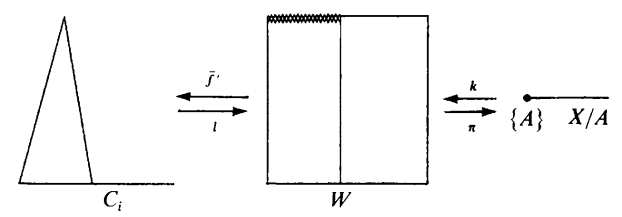
\includegraphics[width=0.8\textwidth]{Figures/DWIJJXNXJNXJUI.png}
        \caption{}
        \label{fig:DWIJJXNXJNXJUI-png}
    \end{figure}
    The map $\overline{f}'$ is induced by
    $\overline{f}$. The map
    $k$ is the "top face" map.
    From this, we see that
    \begin{align*}
        \overline{f}' \circ l 
        &= \id \\
        \pi \circ k 
        &= \id \\
        k \circ \pi 
        &\simeq \id \\
        \overline{f}' \circ k
        &= g \\
        \pi \circ l 
        &= l.
    \end{align*}
   Hence $g h = \overline{f}' k \pi l 
   \simeq \overline{f}' l = \id$. 
\end{proof}


\begin{example}[A non example]
    An example of when the result
    of Theorem 1.6 does not hold is with
    $A = \left\{ 0 \right\} \cup 
    \left\{ \frac{1}{n} \mid n = 1, 2, \ldots \right\} $ 
    and $X = \left[ 0,1 \right] $.
    In this case, $C_{\iota}$ is not homotopy equivalent
    to $X / A$ which is a one-point union of a countably infinite
    sequence of circles with radii going to zero.

    $C_i$ has homeomorphs of circles joined along edges. However,
    the circles do not tend to a point ,so any prospective homotopy
    equivalence $X / A \to C_{\iota}$ would be discontinuous at
    the image of $\left\{ 0 \right\} $ in $X / A$.
\end{example}

\begin{corollary}\label{Cor:Cofibration-Homology}
    If $A \subset X$ is closed and the inclusion
    $A \hookrightarrow X$ is a cofibration, then the map
    $j \colon \left( X, A \right) \to 
    \left( X / A, * \right) $ induces isomorphisms
    \[
    H_* (X,A) \stackrel{\cong}{\to} 
    H_* \left( X / A, * \right) 
    \cong \tilde{H}_* \left( X / A \right) 
    \] 
    and
    \[
    \tilde{H}^{*}(X /A) \cong
    H^{*} (X / A, *) 
    \stackrel{\cong}{\to} H^{*} (X , A).
    \] 
\end{corollary}

\begin{proof}
    We have
    $H_* \left( X/A , *\right) \cong
    H_* \left( C_{\iota}, CA \right) $ by Theorem
    \ref{Thm:2030akKAK}. And since
    $C_{\iota} = X \cup A \times \left[ 0,\frac{1}{2} \right] $ 
    and $CA = A \times \left[ 0,\frac{1}{2} \right] $, where
    we collapse $A \times \left\{ \frac{1}{2} \right\} $ in
    both, and attach  $A \times \left[ 0,\frac{1}{2} \right] $ 
    along $A \times \left\{ 0 \right\} $ in
    $X \cup A \times \left[ 0,\frac{1}{2} \right] $, we obtain
    \[
    H_*(C_{\iota}, CA) \cong
    H_* \left( X \cup A \times \left[ 0,\frac{1}{2} \right] ,
    A \times \left[ 0, \frac{1}{2} \right] \right) 
    \cong H_* (X, A)
    \] 
    since 
    $\left( X \cup A \times \left[ 0,\frac{1}{2} \right] ,
    A \times \left[ 0,\frac{1}{2} \right] \right) 
    \simeq \left( X,A \right) $ by deformation retracting
    $A \times \left[ 0,\frac{1}{2} \right] $ down to
    $A \times \left\{ 0 \right\} \subset X$.
\end{proof}


\subsubsection{Interlude on pointed-spaces and
operations on spaces}

We recall some important constructions:

\begin{definition}[Unreduced Suspension]
    For a space $X$, the \textit{unreduced suspension} 
    $\Sigma X$ is the
    quotient obtained from $X \times I$ by
    collapsing $X \times \left\{ 0 \right\} $ to one
    point and $X \times \left\{ 1 \right\} $ to another
    point.
\end{definition}

\begin{note}
    We have $\Sigma S^{n} = S^{n+1}$.
\end{note}



\begin{definition}[Suspension of a map]
    Given a map
    $f \colon X \to Y$, we can suspend $f$ to
    $\Sigma f \colon \Sigma X \to \Sigma Y$
    by letting $\Sigma f$ be the induced
    map on the quotients:
    \begin{equation*}
    \begin{tikzcd}
        X \times I \ar[r, "f \times \id"] \ar[d]  & Y \times I \ar[d] \\
        \Sigma X \ar[r, "\Sigma f"] & \Sigma Y
    \end{tikzcd}
    \end{equation*}
    
\end{definition}

\begin{definition}[Reduced Suspension]
    For a space $X$, the \textit{reduced suspension}
    $SX$ is the quotient
    \[
    SX = X \times I / \left( X \times \partial I
    \cup \left\{ * \right\} \times I \right) .
    \] 
\end{definition}

\begin{definition}[Reduced Suspension of a map]
    The reduced suspension of a map $f \colon X \to Y$ is
    the induced map on the reduced suspensions of
    $X$ and $Y$ :
    \begin{equation*}
    \begin{tikzcd}
        X \times I \ar[r, "f \times \id"]
        \ar[d] & Y \times I \ar[d] \\
        SX \ar[r, "Sf"] & SY
    \end{tikzcd}
    \end{equation*}
    
\end{definition}

\begin{exercise}[]
    For any homology theory, show that
    there is a natural isomorphism
    $\tilde{H}_I (X) \stackrel{\cong}{\to} 
    \tilde{H}_{i+1} \left( \Sigma X \right) $. Here,
    natural means that for a map $f \colon X \to Y$,
    and its suspension $\Sigma f \colon \Sigma X \to 
    \Sigma Y$, the following diagram commutes:
    \begin{equation*}
    \begin{tikzcd}
        \tilde{H}_i (X) \ar[r, "\cong"] \ar[d, "f_*"]& 
        \tilde{H}_{i+1} \left( \Sigma X \right)
        \ar[d, "(\Sigma f)_*"] \\
        \tilde{H}_i (Y) \ar[r, "\cong"] & \tilde{H}_{i+1}
        \left( \Sigma Y \right) 
    \end{tikzcd}
    \end{equation*}
    
\end{exercise}


\begin{definition}[Wedge Sum/one-point union]
    Given two pointed spaces $(X, x_0), \left( Y, y_0 \right) $,
    we define
    the \textit{wedge sum}  $X \vee Y$ to be
    \[
    X \vee Y = X \sqcup Y / \left( x_0 \sim y_0 \right) ,
    \] 
    i.e., the quotient of the disjoint union identifying
    $x_0$ and $y_0$ to a single point.
\end{definition}

\begin{definition}[Smash Product]
    Inside the product $X \times Y$
    of two pointed space $(X,x_0), (Y,y_0)$,
    we have natural copies of $X$ and $Y$ by
    $X \times \left\{ y_0 \right\} $ and
    $\left\{ x_0 \right\} \times Y$, respectively.
    These two copies intersect only at the point
    $\left( x_0,y_0 \right) $, so their union can
    be identified with
    the wedge sum $X \vee Y$. I.e., $X \vee Y = 
    X \times \left\{ y_0 \right\} \cup 
    \left\{ x_0 \right\} \times Y$. We define
    the \textit{smash product} $X \wedge Y$ to be
    the quotient $X \times Y / X \vee Y$.
\end{definition}


If $f \colon X \to Y$ is a pointed map, then
the reduced mapping cylinder of $f$ is defined
as the quotient space $M_f$ of
$\left( X \times I \right) \cup  Y$ modulo the relations
identifying
$\left( x,0 \right) \sim f(x)$ and the set
$\left\{ * \right\} \times I$ to the base point of $M_f$.\\
The reduced mapping cone is the quotient of the reduced
mapping cylinder $M_f$ obtained by identifying the image of
$X \times \left\{ 1 \right\} $ to a point, the
base point.\\

The circle $S^{1}$ is defined as
$I / \partial I$ with base point $\left\{ \partial I \right\} $.\\
The reduced suspension of a pointed space $X$ is
$SX = X \wedge S^{1}$. It can also be considered
as the quotient space $X \times I / \left( X \times 
\partial I \cup  \left\{ * \right\} \times I\right) $


\begin{definition}[Well-pointed space]
    A base point $x_0 \in X$ is said to be
    \textit{nondegenerate} if the inclusion
    $\left\{ x_0 \right\} \hookrightarrow X$ is a cofibration.
    A pointed Hausdorff space $X$ with nondegenerate
    base point is said to be \textit{well-pointed}.
\end{definition}

It is clear that any manifold or CW-complex satisfies
Theorem \ref{Thm:SJJDHW29WW} with $A$ being any point of
the space. Hence any manifold or CW-complex is
well-pointed.\\

\begin{example}[Pointed space that is not well-pointed]
    Taking the pointed space  $X = 
    \left\{ 0 \right\} \cup  \left\{ \frac{1}{n} \mid 
    n \in \mathbb{N} \right\} $ with base point $0$, this
    space is not well-pointed. This can for example be
    seen because it fails to satisfy Theorem
    \ref{Thm:Retract-cofibration} - any retraction
    would break continuity at
    $\left( 0,1 \right) $.
\end{example}

\begin{example}[]
    If $A \hookrightarrow X$ is a cofibration, then
    $X / A$ with base point $\left\{ A \right\} $ is well-pointed,
    as follows from Theorem \ref{Thm:SJJDHW29WW}.
\end{example}

\begin{theorem}[]
    If $X$ is well-pointed, then so are the reduced
    cone $CX$ and the reduced suspension $SX$. Moreover,
    the collapsing map  $\Sigma X \to SX$, of the unreduced
    suspension to the reduced suspension, is a homotopy
    equivalence.
\end{theorem}

\begin{proof}
    Denote the base point of $X$ by $*$.
    Consider the homeomorphism
    \[
    h \colon \left( I \times I,
    I \times \left\{ 0 \right\} \cup 
\partial I \times I \right) 
\stackrel{\cong}{\to} \left( I \times I, I \times 
\left\{ 0 \right\} \right) 
    \] 
    which clearly exists. For example, take Figure
    \ref{fig:IWIDK01-jpeg}
    \begin{figure}[htpb]
        \centering
        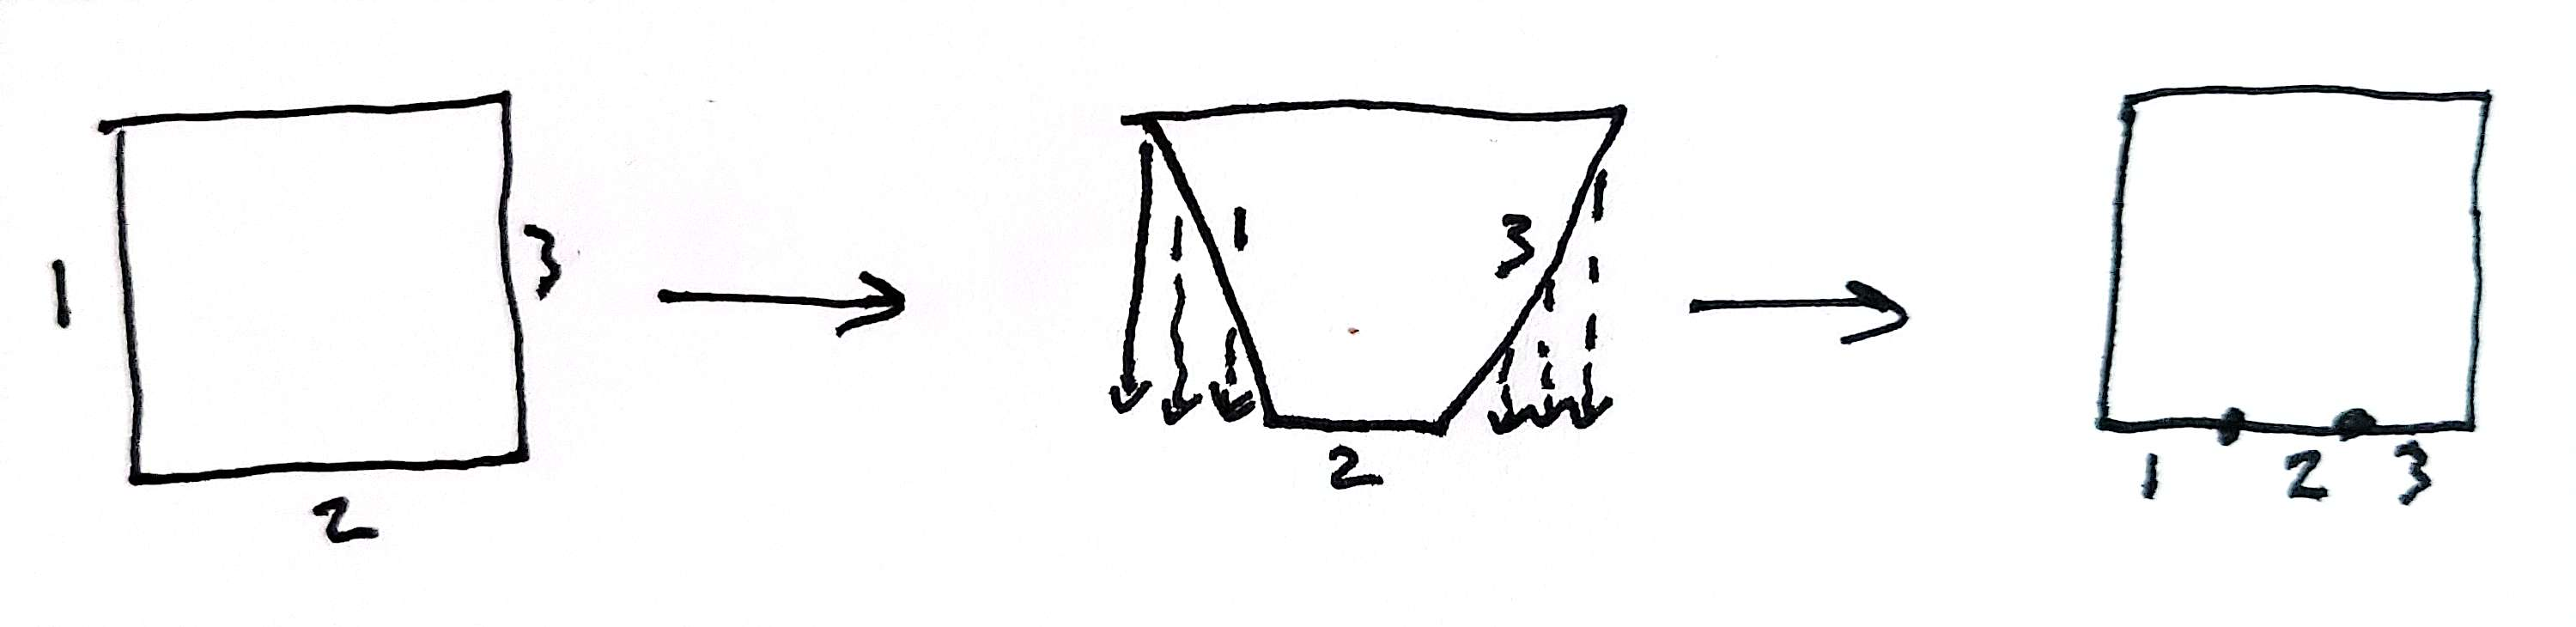
\includegraphics[width=0.5\textwidth]{Figures/IWIDK01.jpeg}
        \caption{}
        \label{fig:IWIDK01-jpeg}
    \end{figure}

    Then the induced homeomorphism
    \[
    \id_X \times h\colon X \times I \times I 
    \stackrel{\cong}{\to} X \times I \times I
    \] 
    carries 
    $X \times I \times \left\{ 0 \right\} \cup 
    X \times \partial I\times I$ to
    $X \times I \times \left\{ 0 \right\} $.
    Hence it takes
    $A = X \times I \times \left\{ 0 \right\} \cup 
    X \times \partial I \times I \cup 
    \left\{ * \right\} \times I \times I$ to
    $X \times I \times \left\{ 0 \right\} 
    \cup \left\{ * \right\} \times I \times I$. 
    Therefore, the pair
    $\left( X \times I \times I, A \right) $ is homeomorphic
    to the pair
    $I \times \left( X \times I, 
    X \times \left\{ 0 \right\} \cup 
\left\{ * \right\} \times I \right) $.
Now, $X$ is well-pointed, so
$X \times \left\{ 0 \right\} \cup 
\left\{ * \right\} \times I$ is a retract of
$X \times I$ by
Theorem \ref{Thm:Retract-cofibration} and the
definition of well-pointed.
It follows that
$A$ is a retract of
$X \times I \times I$.
By another application of
\ref{Thm:Retract-cofibration}, then
the inclusion
$X \times \partial I \cup \left\{ * \right\} \times I
\hookrightarrow X \times I$ is a cofibration. 
Hence the quotient by this,
$SX = X \times I / \left( X \times \partial I
\cup \left\{ * \right\} \times I \right) $ is well-pointed,
using the quotient of the above inclusion.\\
\linebreak
Next consider the homeomorphism
$\left( I \times I, I \times \left\{ 0 \right\} \cup 
\left\{ 1 \right\} \times I \right) 
\stackrel{\cong}{\to} \left( 
I \times I, I \times \left\{ 0 \right\} \right) $ which
can be seen similarly. The induced
homeomorphism
\[
1 \times h \colon X \times I \times I
\stackrel{\cong}{\to} X \times I \times I
\] 
takes
$A:= X \times \left\{ 1 \right\} \times I \cup 
\left\{ * \right\} \times I \times I
\cup X \times I \times \left\{ 0 \right\} $ to
$X \times I \times \left\{ 0 \right\} \cup 
\left\{ * \right\} \times I \times I$.
Thus the pair
$\left( X \times I \times I,
A\right) $ is homeomorphic to
 $I \times \left( X \times I,
 X \times \left\{ 0 \right\} \cup 
\left\{ * \right\} \times I\right) $.
Just as above, we have that
$X \times \left\{ 0 \right\} \cup 
\left\{ * \right\} \times I$ is a retract
of $X \times I$, so
it follows that
$A$ is a retract of $X \times I \times I$. Thus
the inclusion
$X \times \left\{ 1 \right\} \cup 
\left\{ * \right\} \times I \hookrightarrow
X \times I$ is a cofibration, which shows
that $CX = X \times I / \left( X \times \left\{ 1 \right\} 
\cup \left\{ * \right\} \times I\right) $ is
well-pointed.\\
\linebreak
The fact that
$X \times \partial I \cup \left\{ * \right\} \times I
\hookrightarrow X \times I$ is a cofibration
gives that there exists a neighborhood $U$ of
$X \times \partial I \cup 
\left\{ * \right\} \times I$ and a map
$\varphi \colon X \times I \to I$ 
that satisfy Theorem \ref{Thm:SJJDHW29WW}.
We obtain an induced map
$\overline{\varphi }\colon
\Sigma X \to I$ 
which satisfies the same conditions, so
$I \times \times \left\{ * \right\} \times I
\hookrightarrow X \times I / 
\left\{ X \times \left\{ 0 \right\} ,
X \times \left\{ 1 \right\} \right\} = \Sigma X$ is a
cofibration. Now 
Theorem \ref{Thm:2030akKAK} implies
that $\Sigma X \cup CI = C_{\iota} \to \Sigma X / I$ is a homotopy
equivalence.
Hence we obtain
that 
$\Sigma X \simeq
\Sigma X \cup CI \simeq
\Sigma X / I = SX$, via the collapsing map.

\end{proof}


\begin{problem}[]
    Find $H_* \left( \mathbb{P}^2, \mathbb{P}^{1} \right) $ 
    using methods or results from this section.
\end{problem}

\begin{solution}
    Consider $\mathbb{P}^2$ as 
    $S^2$ quotiented by the relation
    $x \simeq -x$. Then
    we can think of  $\mathbb{P}^{1}$ as
    $S^{1} \subset S^{2}$ under this relation.
    We want to show that the inclusion
    $\mathbb{P}^{1} \hookrightarrow \mathbb{P}^2$ is a
    cofibration. 
    Using Theorem \ref{Thm:SJJDHW29WW}, it suffices to
    find a neighborhood $U$ of $\mathbb{P}^{1} \subset 
    \mathbb{P}^2$ and a map $\overline{\varphi } \colon
    \mathbb{P}^2 \to I$ such that
    the conditions of the theorem are satisfied.
    We construct a preliminary map on
    $S^2$ towards this end. 
    Define $\varphi \colon S^2 \to I$ to be
    $\varphi (x) = 
    \min \left\{ 1, 2 \left| x_3 \right|  \right\} $, where
    $x_3$ is the last coordinate of $x$. Since
    $\varphi (x) = \varphi (-x)$, $\varphi $ induces
    a map $\overline{\varphi }\colon
    \mathbb{P}^2 \to I$ such that the diagram
    \begin{equation*}
    \begin{tikzcd}
        S^2 \ar[d] \ar[dr, "\varphi "] & \\
        \mathbb{P}^2 \ar[r, "\overline{\varphi }"] & I
    \end{tikzcd}
    \end{equation*}
    commutes.
    Letting $U$ be the image under the quotient
    map of 
    $\left\{ x \in S^2  \mid 
    \left| x_3 \right| < \frac{1}{2} \right\} $, this
    becomes an open set in $\mathbb{P}^2$ since 
    the above set is saturated with respect to the quotient
    map. It is also clear that
    $U$ and $\overline{\varphi }$ satisfy the conditions of
    the theorem, hence the inclusion
    $\mathbb{P}^{1} \hookrightarrow \mathbb{P}^2$ is a cofibration.
    By Corollary \ref{Cor:Cofibration-Homology}, we
    obtain that
    $H_* \left( \mathbb{P}^2, \mathbb{P}^{1} \right) 
    \cong \tilde{H}_* \left( \mathbb{P}^2 / \mathbb{P}^{1} \right) $.
    But $\mathbb{P}^2 / \mathbb{P}^{1} \cong
    S^{2}$, so
    $H_* \left( \mathbb{P}^2, \mathbb{P}^{1} \right) 
    \cong \tilde{H}_* \left( S^2 \right)$.
    Now simply recall that
    \[
    \tilde{H}_p \left( S^2 \right) 
    \cong
    \begin{cases}
        \mathbb{Z},& p = 2\\
        0,& p \neq 2.
    \end{cases}
    \] 
    \qed
\end{solution}

\begin{problem}[]
    Find $H_*\left( T^2,
    \left\{ * \right\} \times S^{1} \cup 
S^{1} \times \left\{ * \right\} \right) $ using
methods from this section.
\end{problem}

\begin{solution}
    If we can show that the inclusion
    $A:= \left\{ * \right\} \times S^{1} \cup 
    S^{1} \times \left\{ * \right\} \hookrightarrow
    T^2$ is a cofibration, then
    we will again obtain that
    $H_* (T^2, A) \cong
    \tilde{H}_* \left( T^2 / A \right) \cong
    \tilde{H}_* \left( S^2 \right) $.
    But we have a CW-structure on the
    torus given by the square with identified sides.
    With this identificaiton, $A$ simple becomes
    the $1$-skeleton, hence it is a subcomplex, so
    by Corollary \ref{Cor:Subcomplex-Cofibration}, 
    the inclusion $A \hookrightarrow T^2$ is a cofibration.
    This finishes the solution. \qed
\end{solution}

\begin{problem}[]
    For a space $X$, consider the pair
    $\left( CX, X \right) $. What do the results of this
    section tell you about the homology of these, and related,
    spaces?
\end{problem}


\begin{solution}
    We can define a map
    $\varphi \colon CX \to I$ by
    $\varphi (x,t) = t$. Choosing
    $A = X = X \times \left\{ 0 \right\} \subset 
    CX$ and
    $U = CX - \left\{ v \right\} $ where
    $v$ is the vertex, this satisfies the
    conditions in Theorem \ref{Thm:SJJDHW29WW} 
    ($H$ can be defined by
    $H((x,t_0),t) = \left( x,t_0 \right) (1-t)
    + (x,0) t$).
    Hence the inclusion
    $X \hookrightarrow CX$ is a cofibration, so we
    know that
    $H_* \left( CX, X \right) 
    \cong \tilde{H}_* \left( CX / X \right) $.
    Similarly, one can
    show that the inclusion
    $X \hookrightarrow \Sigma X$ is a cofibration, so
    $H_* \left( \Sigma X , X \right) 
    \cong \tilde{H}_* \left( \Sigma X / X \right) 
    \cong \tilde{H}_* \left( 
    \Sigma X \vee \Sigma X \right) $ and
    $H_*\left( SX, X \right) 
    \cong \tilde{H}_* \left( SX \vee SX \right) $.
\end{solution}


\begin{problem}[]
    If $f \colon A \to X$ is a cofibration then show that
    $f$ is an embedding. If $X$ is also Hausdorff,
    then show that $f(A)$ is closed in $X$.
\end{problem}

\begin{proof}
    Since $f$ is a cofibration, the following diagram
    can be filled out, inducing a map
    $g \colon X \times I \to M_f$ :
    \begin{equation*}
    \begin{tikzcd}
        A \times \left\{ 0 \right\} \ar[dd, "f \times \id"] 
        \ar[rr, hookrightarrow] & & A \times I \ar[dd, "f \times 
        \id"] \ar[dl, "q"] \\
                                & M_f & \\
        X \times \left\{ 0 \right\} \ar[ur, "q"] 
        \ar[rr, hookrightarrow]& & X \times I 
        \ar[ul, "g"]
    \end{tikzcd}
    \end{equation*}
    By construction, we have that
    $q \colon A \times \left\{ 1 \right\} 
    \hookrightarrow M_f$ is an embedding, so
    letting $l \colon
    q \left( A \times \left\{ 1 \right\}  \right) 
    \to A \times \left\{ 1 \right\} $ be the inverse map,
    we have
    $l \circ g|_{f(A) \times \left\{ 1 \right\} } 
    \circ \left( f \times \id \right) 
    = \id_{A \times \left\{ 1 \right\} }$.
    Likewise,
    $\left( f \times \id \right) 
    \circ l \circ g|_{f(A) \times \left\{ 1 \right\} }$,
    since $g \left( f(a), t \right) 
    = q(a,t)$, we have that
    $l \circ g|_{f(A) \times \left\{ 1 \right\} }
    (f(a),1) = (a,t)$, hence
    $\left( f \times \id \right) 
    \circ l \circ g|_{f(A) \times \left\{ 1 \right\} }
    = \id_{f(A) \times \left\{ 1 \right\} }$.
    Therefore,
    $f \times \id$ is a homeomorphism
    $A \times \left\{ 1 \right\}  \stackrel{\cong}{\to} 
    f(A) \times \left\{ 1 \right\} $, so
    $f \colon A \stackrel{\cong}{\to} f(A)$ is a homeomorphism.\\
    \linebreak
    By Lemma \ref{Lemma:Cofibration-Inclusion-2} and
    Theorem \ref{Thm:Retract-cofibration}, we
    have that there exists a retraction
    $r \colon X \times I \to 
    X \times \left\{ 0 \right\} \cup 
    f(A) \times I$.

    \begin{lemma}[]
         If a space $X$ is Hausdorff and
          there exists a retraction
          $r \colon X \to A$, then $A$ is closed.
    \end{lemma}

    \begin{proof}
        Let
        $x \in X -A$ be a limit point of $A$. Let
        $U ,V$ be open disjoint neighborhoods of
        $x$ and $r(x)$. Then
        $r^{-1}(V)$ is open and contains $x$, so
        let $U' = U \cap r^{-1}(V)$.
        Now $U \cap A \cap r^{-1}(V) = \varnothing$ since
        otherwise $U \cap A = r\left( U \cap A \right) 
        \subset V$ contradicting $U \cap V = \varnothing$.
        But then $U'$ is an open neighborhood of $x$
        that is disjoint from $A$, contradicting $x$ being
        a limit point of $A$.
        Thus $\overline{A} = A$.
    \end{proof}

    Using this Lemma, we find that since
    $X \times I$ is Hausdorff and
    $r \colon X \times I \to X \times \left\{ 0 \right\} 
    \cup f(A) \times I$ is a retraction,
    $X \times \left\{ 0 \right\} \cup 
    f(A) \times I$ is closed in
    $X \times I$.
    Now,
    $f(A) \times \left\{ 1 \right\} 
    = X \times \left\{ 1 \right\} 
    \cap \left( X \times \left\{ 0 \right\} \cup 
    f(A) \times I\right) $, so
    since $X \times \left\{ 1 \right\} $ is closed
    in $X \times I$,
    $f(A) \times \left\{ 1 \right\} $ 
    is by definition closed in 
    $X \times \left\{ 0 \right\} \cup 
    f(A) \times I$ in the subspace topology. Hence
    it is also closed in $X \times I$.
    Now we use another lemma:
    \begin{lemma}[]
        If $Y$ is a compact space, then
        the projection $X \times Y \to X$ is a closed map.
    \end{lemma}
    \begin{proof}
        Let $W \subset X \times Y$ be closed and
        set $W' = X \times Y -W$.
        Note that $x_0 \in \pi_X (W)$ if and only
        if $\exists y_0 \in Y$ such that
        $(x_0,y_0) \in W$. Thus
        $x_0 \not\in \pi_X(W)$ if and only if
        $\left\{ x_0 \right\} \times Y \subset 
        W'$.

        By the tube lemma,
        $x_0 \not\in \pi_X (W)$ if and only if
        $W'$ contains some tube
        $N \times Y$ about $\left\{ x_0 \right\} \times Y$ 
        where $N$ is an open neighborhood of $x_0$ in $X$. 
        But then
        $N = \pi(N \times Y) \subset 
        X - \pi(W)$ is an open neighborhood of $x_0$ in
        $X - \pi(W)$. Hence
        $X - \pi(W)$ is open, so $\pi(W)$ is
        closed.
    \end{proof}
    Noting that
    $\left\{ 1 \right\} \subset I$ is compact,
    we can apply this Lemma to
    $f(A) \times \left\{ 1 \right\} $ to obtain that
    $f(A)$ is closed in $X$.
    This completes the proof.

\end{proof}

\newpage
\begin{problem}[]
    Let $\iota \colon A \hookrightarrow X$,
    the inclusion of $A$ in $X$, be a cofibration and
    $A$ be a contractible space. Show that the
    quotient map $X \to X / A$ is a homotopy equivalence.
\end{problem}

\begin{proof}
    Let
    $H \colon A \times I \to A$ be the contraction of
    $A$ where
    $H(a,0) = a$ and $H(a,1) = a_0 \in A$.
    Consider the diagram
    \begin{equation*}
    \begin{tikzcd}
        A \times \left\{ 0 \right\} \ar[dd, "\iota \times \id"]
        \ar[rr] 
        & &
        A \times I \ar[dd, "\iota \times \id"] \ar[dl, "H"] \\
                                                    & X&\\
        X \times \left\{ 0 \right\} \ar[rr] \ar[ru,"\id"]
                                                    & & X \times I
        \ar[ul, "\tilde{H}"] 
    \end{tikzcd}
    \end{equation*}
    Then since 
    $\tilde{H}(a,t) \in A$ for all $t$,
    the composition $q \tilde{H} \colon X \times I \to X / A$ sends
    $A$ to a point at all times, hence factors as
    $X \times I \stackrel{q \times \id}{\to} X / A \times I
    \to X / A$. Denote the
    latter map by $\overline{H} \colon 
    X / A \times I \to X / A$. Then
    $q \tilde{H} = \overline{H} \left( q \times \id \right) $.
    When $t = 1$, we have
    $\tilde{H}\left( A,1 \right) $ equal to a point, so
    $\tilde{H}\left( -,1 \right) $ induces a map
    $g \colon X / A \to X$ with $g q = \tilde{H}
    \left( -,1 \right) $.
    It follows that
    $qg = \overline{H}(-,1)$ since
    $qg\left( \overline{x} \right) 
    =qg q(x) = q \tilde{H}(x,1) 
    = \overline{H} \left( q(x),1 \right) =
    \overline{H}\left( \overline{x},1 \right) $.
    Now the maps $g$ and $q$ are inverse homotopy
    equivalences since
    $gq = \tilde{H}(-,1) \simeq
    \tilde{H}(-,0) = \id_X$ and
    $qg = \overline{H}(-,1) \simeq
    \overline{H}(-,0) = \id_{X / A}$.
\end{proof}

\subsubsection{Some Applications of the HEP}

\begin{proposition}[]\label{Prop:HEP-Homotopy-Equivalence}
    Suppose $\left( X,A \right) $ and
    $\left( Y,A \right) $ satisfy the HEP, and 
    $f \colon X \to Y$ is a homotopy equivalence
    with $f |_{A} = \id$. Then $f$ is a homotopy equivalence
    $\rel A$.
\end{proposition}

\begin{corollary}
    If $\left( X,A \right) $ satisfy the HEP and the
    inclusion $A \hookrightarrow X$ is a homotopy equivalence,
    then $A$ is a deformation retract of $X$.
\end{corollary}

\begin{corollary}
    A map $f \colon X \to Y$ is a homotopy equivalence
    if and only if $X$ is a deformation retract of the
    mapping cylinder $M_f$. Hence, two space $X$ and 
    $Y$ are homotopy equivalence if and only if
    there is a third space containing both $X$ and
    $Y$ as deformation retracts.
\end{corollary}
